% Created 2024-10-05 Sat 20:05
% Intended LaTeX compiler: pdflatex
\documentclass[11pt]{article}
\usepackage[utf8]{inputenc}
\usepackage[T1]{fontenc}
\usepackage{graphicx}
\usepackage{longtable}
\usepackage{wrapfig}
\usepackage{rotating}
\usepackage[normalem]{ulem}
\usepackage{amsmath}
\usepackage{amssymb}
\usepackage{capt-of}
\usepackage{hyperref}
\date{\today}
\title{}
\hypersetup{
 pdfauthor={},
 pdftitle={},
 pdfkeywords={},
 pdfsubject={},
 pdfcreator={Emacs 29.4 (Org mode 9.7.11)}, 
 pdflang={English}}
\begin{document}

\section*{Question Paper}
\label{sec:org81701c2}

\subsection*{Delhi Public School}
\label{sec:org1678958}
\subsection*{Gurugram I Sector 67A}
\label{sec:orge7ad3d6}

\subsection*{HALF YEARLY ASSESSMENT}
\label{sec:org79ed952}
\subsection*{SESSION: 2024-25}
\label{sec:orge16b49c}

\subsection*{NAME:}
\label{sec:org32dd2f4}
\subsection*{CLASS: VII}
\label{sec:orgcc6ce39}
\subsection*{ROLL NO:}
\label{sec:org146fc5f}

\subsection*{DATE: 17th September, 2024}
\label{sec:orgcaadcf2}
\subsection*{SUBJECT: Mathematics}
\label{sec:orge9a69bc}
\subsection*{M.M: 80}
\label{sec:org3241880}
\subsection*{DURATION: 3 hrs}
\label{sec:org915597d}

\subsection*{INSTRUCTIONS:}
\label{sec:org51caf99}

\begin{itemize}
\item Read the question paper carefully.
\item All the questions are mandatory.
\item This question paper consists of 33 questions and 5 printed pages.
\item Number your answers correctly according to the questions.
\item Do not write any information on the question paper.
\end{itemize}
\section*{Section A (10 Marks)}
\label{sec:org2cc35b1}

\subsection*{Q.1}
\label{sec:orgbd7eca0}
The value of 1.3 × 3.1 is
\begin{itemize}
\item a. 4.03
\item b. 0.403
\item c. 4.0339
\item d. 0.0403
\end{itemize}
\subsection*{Q.2}
\label{sec:orgbcfab16}
The number of angles formed, when two lines intersect, is
\begin{itemize}
\item a. 5
\item b. 4
\item c. 2
\item d. 6
\end{itemize}
\subsection*{Q.3}
\label{sec:org222c736}
What is the product of the largest and the smallest fraction from the following list?

9/11
3/11
7/11
5/11
10/11
6/11
Options:

\begin{itemize}
\item a. 18/121
\item b. 30/121
\item c. 35/121
\item d. 90/121
\end{itemize}
\subsection*{Q.4}
\label{sec:org81709ba}
The solution of the equation \(3x+4=25\) is
\begin{itemize}
\item a. 7
\item b. 8
\item c. 9
\item d. 6
\end{itemize}
\subsection*{Q.5}
\label{sec:org6ad17ca}
Find the fraction of 3 km to 300 m.
Options:
\begin{itemize}
\item a. 1/100
\item b. 10/1
\item c. 1/10
\item d. 100/1
\end{itemize}
\subsection*{Q.6}
\label{sec:org9e4d866}
\(-5+9+(-5)+(-10)+(7)\) is equal to
\begin{itemize}
\item a. 13
\item b. -13
\item c. 10
\item d. -10
\end{itemize}
\subsection*{Q.7}
\label{sec:orga268f8e}
In the adjoining figure, if AB = PQ and BC = CQ, then find the measure of angle CPQ.
\begin{center}
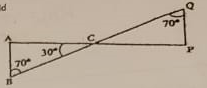
\includegraphics[width=.9\linewidth]{./maths7.png}
\end{center}
\begin{itemize}
\item a. 30°
\item b. 90°
\item c. 80°
\item d. 60°
\end{itemize}
\subsection*{Q.8}
\label{sec:org6064a78}
Mean of 11, 10, 12, 12, 9, 10, 14, 12, 9 is
\begin{itemize}
\item a. 20
\item b. 10
\item c. 14
\item d. 11
\end{itemize}
\subsection*{Q.9}
\label{sec:orgea7cc87}
An expression remains the same, when the expressions on the left and on the right are interchanged.
\begin{itemize}
\item a. Expression
\item b. Equation
\item c. Variable
\item d. Constant
\end{itemize}
\subsection*{Q.10}
\label{sec:org9bfa11d}
Number of acute angles in the following figure is
\begin{itemize}
\item a. 3
\item b. 1
\item c. 4
\item d. 2
\end{itemize}
\begin{center}
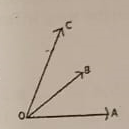
\includegraphics[width=.9\linewidth]{./maths10.png}
\end{center}
\section*{Section B (12 Marks)}
\label{sec:org3cfa98d}

\subsection*{Q.11}
\label{sec:orgba16b76}
Find the value of x in the adjacent figure and state the property that is used to find the value.
\begin{itemize}
\item a. 30°
\item b. 60°
\item c. 45°
\item d. 50°
\end{itemize}
\begin{center}
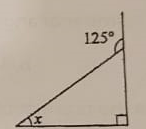
\includegraphics[width=.9\linewidth]{./maths11.png}
\end{center}
\subsection*{Q.12}
\label{sec:org79a2bfd}
If 28 trousers of equal size can be made from 63 m of cloth, what length of cloth is required for one trouser?
\subsection*{Q.13}
\label{sec:orgc395458}
Calculate the mean of the first five prime numbers.
\subsection*{Q.14}
\label{sec:orgca694f4}
If 2x-1=x+2, then what is the value of x?
\subsection*{Q.15}
\label{sec:orgb04a432}
Calculate median and mode for the following data:
38, 45, 46, 12, 34, 87, 78, 12, 65, 35, 19, 34, 55, 67, 81, 12, 56, 98, 1, 49, 23, 50
\subsection*{Q.16}
\label{sec:orged25d50}
Raju owns a plot which is 1 acre in size. If the value of land in his area is ₹48,000 per acre, what is the value of his plot?
\section*{Section C (30 Marks)}
\label{sec:org6e15bde}

\subsection*{Q.17}
\label{sec:org5d73e89}
In a family, the consumption of wheat is 4 times that of rice. The total consumption of the two cereals is 80 kg. Find the quantities of rice and wheat consumed in the family.
\subsection*{Q.18}
\label{sec:orgff42e92}
The given data is arranged in ascending order. The sum of mode and median of the given data is 15. Find the value of y.
\(y-1, y-1, y+1, y+4, 2y+1, 3y, 4y\)
\subsection*{Q.19}
\label{sec:org76ec030}
In the given adjacent figure, △QPR is a right-angled triangle with angle QPR = 70°.
\begin{itemize}
\item i) Find the value of y
\item ii) Find the value of x
\item iii) Find the value of z
\end{itemize}
\begin{center}
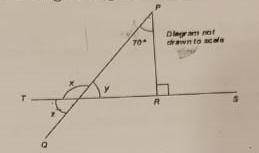
\includegraphics[width=.9\linewidth]{./maths19.png}
\end{center}
\subsection*{Q.20}
\label{sec:org477506b}
A square and an equilateral triangle have a side in common. If the side of the triangle is 4/3 cm long, find the perimeter of the adjacent figure.
\begin{center}
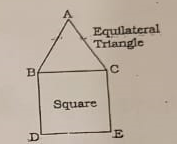
\includegraphics[width=.9\linewidth]{./maths20.png}
\end{center}
\subsection*{Q.21}
\label{sec:org1f95087}
In the given adjacent figure, EV, FK, and GS are the medians of the triangle EFG. Find the value of:
\begin{itemize}
\item i) FS
\item ii) KG
\item iii) FV
\end{itemize}
\begin{center}
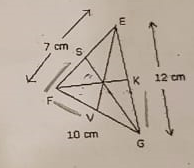
\includegraphics[width=.9\linewidth]{./maths21.png}
\end{center}
\subsection*{Q.22}
\label{sec:org7d7d10d}
A shopkeeper earns a profit of ₹1 by selling one pen and incurs a loss of 40 paise per pencil while selling pencils of her old stock. In a particular month, she incurs a loss of ₹5. In this period, she sold 45 pens. How many pencils did she sell in this period?
\subsection*{Q.23}
\label{sec:org460101b}
A car covers a distance of 89.1 km in 2.2 hours. What is the average distance covered by it in 1 hour?
\subsection*{Q.24}
\label{sec:org5c02ef7}
"5 added to three-fifth of a number gives 14/3".
\begin{itemize}
\item i) Write the equation for the above statement.
\item ii) Solve the equation and find the number.
\end{itemize}
\subsection*{Q.25}
\label{sec:org355c39a}
In a class test containing 15 questions, 4 marks are given for every correct answer and (-2) marks are given for every incorrect answer.
\begin{itemize}
\item i) Gurpreet attempts all questions but only 9 of her answers are correct. What is her total score?
\item ii) One of her friends attempted all questions and got only 5 answers correct. What will be her score?
\end{itemize}
\subsection*{Q.26}
\label{sec:org3aea945}
If RO is perpendicular to PT in the adjacent figure, find the measure of angle 1 and angle 2.
\begin{center}
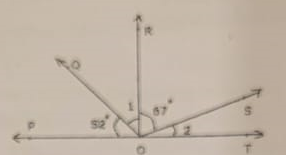
\includegraphics[width=.9\linewidth]{./maths26.png}
\end{center}
\section*{Section D (28 Marks)}
\label{sec:org3bc8f7a}

\subsection*{Q.27}
\label{sec:orge82bc73}
Simplify and reduce to standard form:
\begin{center}
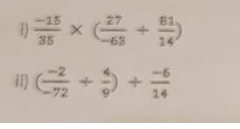
\includegraphics[width=.9\linewidth]{./maths27.png}
\end{center}
\subsection*{Q.28}
\label{sec:org9279d7a}
The data given below shows the production of motor bikes in a factory for some months of two consecutive years.

\begin{center}
\begin{tabular}{lrr}
Months & 2023 & 2024\\
\hline
February & 2700 & 2800\\
May & 3200 & 4500\\
August & 6000 & 4800\\
October & 5000 & 4800\\
December & 4200 & 5200\\
\end{tabular}
\end{center}

\begin{itemize}
\item i) Draw a double bar graph using appropriate scale to depict the above information.
\item ii) In which year was the total output the maximum?
\end{itemize}
\subsection*{Q.29}
\label{sec:org6342a23}
The foot of a ladder is 6 m away from a wall, and its top reaches 8 m above the ground.
\begin{itemize}
\item i) Find the length of the ladder.
\item ii) If the ladder is shifted in such a way that its foot is 8 m away from the wall, to what height does its top reach?
\end{itemize}
\subsection*{Q.30}
\label{sec:org16a5e22}
\begin{itemize}
\item i) Raju's father's age is 5 years more than three times Raju's age. Find Raju's age, if his father is 44 years old.
\item ii) Find a number, such that one-fourth of the number is 3 more than 7.
\end{itemize}
\subsection*{Q.31}
\label{sec:org3f121e2}
There are four containers that are arranged in the ascending order of their heights. If the height of the smallest container given in the below figure is expressed as x = 10.5 cm, find the height of the largest container (x).
\begin{center}
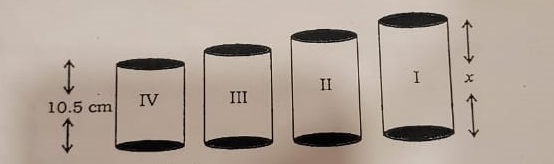
\includegraphics[width=.9\linewidth]{./maths31.png}
\end{center}
\subsection*{Q.32}
\label{sec:orgb578b96}
Find the value of x in the adjacent figure.
\begin{center}
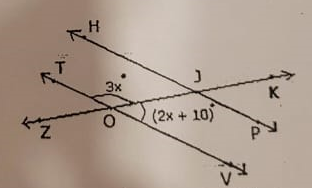
\includegraphics[width=.9\linewidth]{./maths32.png}
\end{center}
\subsection*{Q.33}
\label{sec:org9d72099}
A tree is broken at a height of 5 m from the ground, and its top touches the ground at a distance of 12 m from the base of the tree. Find the original height of the tree.
\end{document}
